\chapter{简介}
倒立摆系统是一个非线性自然不稳定系统,是进行控制理论教学及开展各种控制实验的理想实验平台。许多抽象的控制概念如控制系统的稳定性、可控性、系统收敛速度和系统抗干扰能力等,都可以通过倒立摆系统直观的表现出来。对其基础的理论控制以及算法的学习都有十分巨大的帮助。由于倒立摆本身所具有的高阶次,不稳定,多变量。非线性,和强耦合性,许多现代控制理论的研究人员一直将它作为典型的研究对象,不断从中发掘新的控制策略和控制算法,相关的科研成果在航天科技和机器人学方面获得广阔的应用。

本文通过两种不同的控制方法,即LQR控制方法与模糊控制方法,对直线一级倒立摆实现对手动的加速度脉冲输入的稳定性。其中,实验所用的倒立摆为固高科技公司的直线一级摆:直线倒立摆在直线运动模块(小车)上装有摆杆和角度编码器,直线运动模块有一个自由度,在伺服电机的驱动下可以沿导轨水平运动,如图\cref{fig:realthing}所示。通过相关方法的处理,倒立摆能够通过调节位移和角度,保证对一定范围内扰动的鲁棒性,并最终实现摆杆竖直位置的保持。通过两种方法实验结果的比较,我们进一步得出了两种方法的优劣,并分析出了产生差异的原因。本文的主要贡献有:
  \begin{itemize}
    \item 分别利用LQR控制方法和模糊控制方法建立了直线一级倒立摆的控制系统;
    \item 通过比较LQR控制方法和模糊控制方法的效果,分析了两者的优劣。
  \end{itemize}

\begin{figure}[hbpt]
\centering
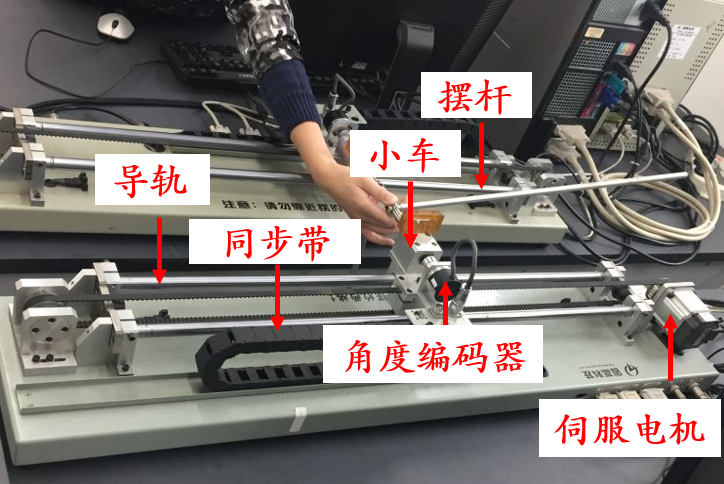
\includegraphics[width=12cm]{realthing.png}
\caption{倒立摆系统}\label{fig:realthing}
\end{figure}



